\section*{Exercice 126 -- Matrice d'inertie}
\setcounter{exo}{0}
%Banque PT SI A 2009

Les galets 2 et 3 sont de masses identiques $m_2$ et de centres d’inertie respectifs $G_2$ et $G_3$. Le balancier 1 est
de masse $m_1$ et de centre d’inertie $O$ (la tige de $G_3H$ étant de masse négligeable). La géométrie simplifiée,
adoptée pour la détermination préalable des caractéristiques d'inertie, est décrite sur la figure suivante.
Les solides 1, 2 et 3 sont supposés homogènes.

\begin{center}
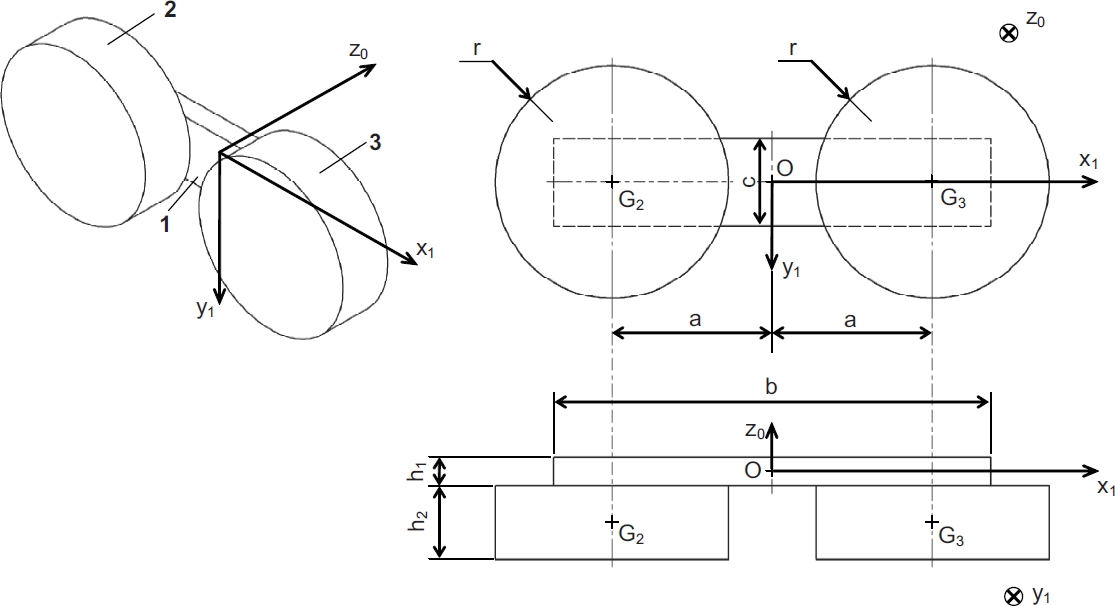
\includegraphics[width=\linewidth]{986_01}%
\end{center}


\subparagraph{}
\textit{Donner la forme de la matrice d’inertie du solide 1 au point $O$ dans la base
$\base{x_1}{y_1}{z_1}$. On justifiera la réponse.}
\ifprof
\begin{corrige}
\end{corrige}
\else
\fi

\subparagraph{}
\textit{Exprimer littéralement le moment d’inertie $C_1$ du solide 1 par rapport à l’axe $\axe{O}{z_0}$
 en fonction de la masse $m_1$ et de ses dimensions.}
\ifprof
\begin{corrige}
\end{corrige}
\else
\fi

\subparagraph{}
\textit{Donner la forme de la matrice d’inertie du solide 2 au point $G_2$ dans la base $\base{x_1}{y_1}{z_0}$. On justifiera la réponse.}
\ifprof
\begin{corrige}
\end{corrige}
\else
\fi

\subparagraph{}
\textit{Exprimer littéralement le moment d’inertie $C_2'$ du solide 2 par rapport à l’axe $\axe{G_2}{z_0}$, en fonction de la masse $m_2$ et de ses dimensions.}
\ifprof
\begin{corrige}
\end{corrige}
\else
\fi

\subparagraph{}
\textit{Exprimer littéralement le moment d’inertie $C_2'$ du solide 2 par rapport à l’axe $\axe{O}{z_0}$ en fonction de la masse $m_2$ et de ses dimensions.}
\ifprof
\begin{corrige}
\end{corrige}
\else
\fi
%
%\subparagraph{}
%\textit{}
%\ifprof
%\begin{corrige}
%\end{corrige}
%\else
%\fi

\begin{enumerate}
\item $\inertie{O}{1}=\matinertie{A_1}{B_1}{C_1}{0}{0}{0}{\base{x_1}{y_1}{z_0}}$.
\item $C_1 = \dfrac{m_1}{12}\left( b^2 + c^2\right)$.
\item $\inertie{G_2}{1}=\matinertie{A_2}{B_2}{C_2}{0}{0}{0}{\base{x_1}{y_1}{z_0}}$.
\item $C'_2 = m_2 \dfrac{r^2}{2}$.
\item $C_2 = m_2\left(\dfrac{r^2}{2}+a^2\right)$.
\end{enumerate}
